\documentclass[../../main.tex]{subfiles}

\graphicspath{{\subfix{../../immagini/}}}

\begin{document}
    Nell'ambito dell'apprendimento supervisionato, come brevemente introdotto nello scorso paragrafo, l'obiettivo è, una volta identificata la classe del problema su cui voglio lavorare, progettare un agente in grado di risolvere tale problema, nello specifico l'agente incaricato avrà a disposizione un dataset, che prende il nome di \textit{training set}, contenente una serie elementi che potrà osservare al fine di riuscire a lavorare anche su nuove istanze mai osservate in precedenza.

    Formalmente, dato un \textit{training set} composto da $N$ elementi nella forma:
    \[(x_1, y_1), (x_2, y_2), \dots, (x_N, y_N)\]
    con ogni $y_i$ generato da una funzione ignota $y = f(x)$, l'obiettivo è trovare una funzione $h$, detta funzione \textit{d'ipotesi}, o modello, che approssimi in modo accettabile la vera funzione $f$.

    L'obiettivo è quindi ricercare nello spazio di tutte le possibili funzioni d'ipotesi una che approssimi la funzione $f$, \textit{anche su nuovi esempi non appartenenti al training set}, si dice in questo caso che $h$ è in grado di \textit{generalizzare}.

    Esistono diverse \textit{classi di funzione d'ipotesi}:
    \begin{itemize}
        \item Funzioni lineari
        \item Funzioni polinomiali grado N
        \item Funzioni sinusoidali
        \item Funzioni esponenziali
    \end{itemize}

    A prescindere dal tipo di classe utilizzata avrò una serie di \textit{parametri}, ad esempio nel caso di una funzione lineare avrei:
    \[h(\boldsymbol{x}) = w_0 + w_1x_1 + \dots + w_nx_n\]
    L'obiettivo è quindi \textit{fittare} la funzione d'ipotesi sui dati: trovare l'insieme di parametri che allineano il più possibile la funzione $h$ con i dati presenti nel training set. 

    A seconda di come la funzione $f$ è definita esistono due principali tipi di apprendimento supervisionato: nel caso in cui $f$ abbia come codominio $\mathbb{R}$ sono in un problema di \textit{regressione}, se invece $f$ ha un codominio con un numero discreto e finito di elementi (Quindi assegna un'\textit{etichetta} ad ogni elemento dell'insieme di training) allora parlo di problema di \textit{classificazione}.

    Esistono in generale diversi algoritmi nelle due tipologie di problemi appena descritte che differiscono principalmente per la loro \textit{espressività}, ovvero la capacità di rappresentare determinati pattern di dati. Importante notare come molti algoritmi possano essere sfruttati sia nell'ambito della classficazione che in quello della regressione.\\
    Mi concentro brevemente, a scopo esemplificativo, sulla \textit{regressione lineare} per problemi di regressione e sulla \textit{regressione logistica} per problemi di classificazione per poi passare, nel prossimo paragrafo, alla descrizione delle \textit{reti neurali}, utilizzate poi negli esperimenti sui filtri.

    \subsubsection{Regressione}

    Nel caso della regressione la funzione $f$ da approssimare è una funzione continua, come già accennato in precedenza sono diversi i metodi utilizzabili in problemi di questo tipo, per citarne alcuni: \textit{regressione lineare, regressione polinomiale, random forest, support vector machines ...} approcci che si differenziano principalmente per la complessità della funzione $h$ con conseguenti differenze nelle capacità di approssimazione di $f$.

    \begin{wrapfigure}{L}{0.5\textwidth}
        \begin{center}
            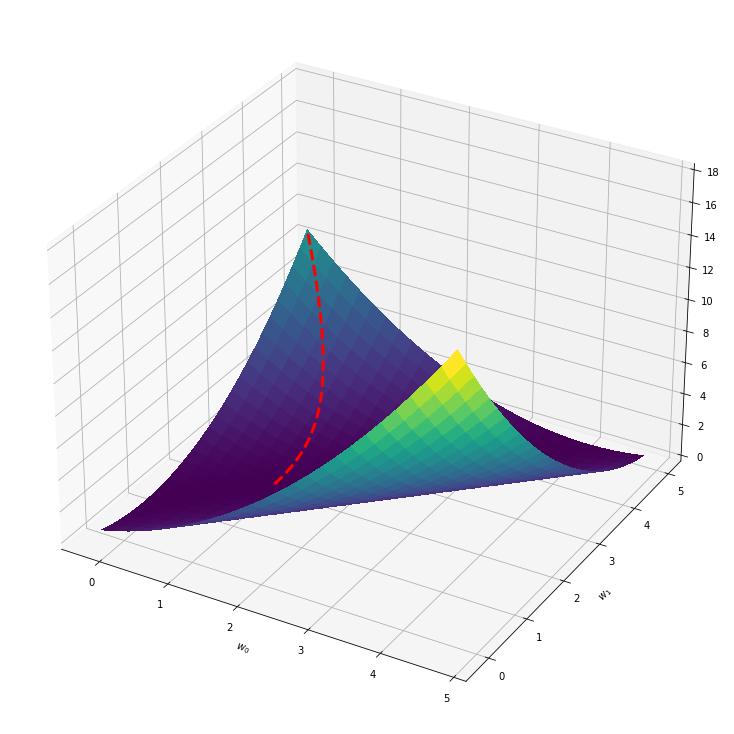
\includegraphics[width = 0.48\textwidth]{immagini/4_1/loss_function.png}
        \end{center}
        \caption{Esempio del funzionamento dell'algoritmo del gradiente utilizzato per aggiornare il valore dei pesi: noto come il valore della funzione di perdita diminuisca all'aumentare del numero di iterazioni fino ad arrivare a convergenza}
        \label{fig:gradient_descent}
    \end{wrapfigure}

    Mi concentro su uno dei metodi più semplici per ragionare su problemi di regressione: la \textit{regressione lineare}:
    
    Parto quindi da una funzione d'ipotesi definita come:
    \[h(\boldsymbol{x}) = w_0 + w_1x_1 + w_2x_2 + \dots + w_nx_n = \boldsymbol{w^T x}\]
    Il problema in questo caso viene detto di \textit{regressione lineare multi-variata}; l'idea è quella di sfruttare gli elementi dell'insieme di training a disposizione per trovare un vettore dei parametri $\boldsymbol{w}$ che permetta di minimizzare, per ognuno degli $y_i$, una funzione, chiamata di \textit{perdita}, definita come la differenza tra $y_i$ e $h(x_i)$; di fatto quindi questa funzione quantifica l'errore commesso dal modello.
    
    Posso definire la funzione di perdita in diversi modi, in questo caso considero una funzione di perdita quadratica:
    \[L(\boldsymbol{w}) = \sum_{j=1}^N(y_j - h(\boldsymbol{x_j}))^2\]
    Per minimizzare la funzione è necessario trovare dei parametri tali per cui la derivata di $L$, in funzione di tali parametri, sia pari a 0:
    \[\frac{\partial}{\partial w} L(\boldsymbol{w}) = 0\]

    Nel caso della regressione lineare l'approccio più semplice è di risolvere analiticamente la derivata al fine di ricavare una funzione generale con cui calcolare direttamente il valore di ognuno dei parametri, prendendo ad esempio il caso più semplice in cui $h$ è in una sola variabile (\textit{regressione univariata}) ottengo le seguenti derivate:
    \[
    \begin{dcases}
        w_0 = & \frac{\sum_{i=1}^N z_i - w_1 \sum_{i=1}^N}{N}\\
        w_1 = & \frac{N(\sum_{i=1}^N z_ix_i) - \sum_{i=1}^N z_i \sum_{i=1}^N x_i}{N(\sum_{i=1}^N x_i^2 - (\sum_{i=1}^N x_i)^2)} 
    \end{dcases}    
    \]
    Non sempre però un approccio di questo tipo è possibile: non sempre infatti esiste una soluzione in forma chiusa della funzione $L$, in casi di questo tipo solitamente si ricorre ad un approccio \textit{iterativo} più generale (https://stats.stackexchange.com/questions/23128/solving-for-regression-parameters-in-closed-form-vs-gradient-descent) con algoritmi che sfruttano il gradiente della funzione $L$, nel nostro caso utilizzeremo un algoritmo di \textit{discesa del gradiente} (Figura \ref{fig:gradient_descent}), in quanto l'obiettivo è di \textit{minimizzare} il valore della perdita.

    Intuitivamente l'algoritmo lavora non più sulla perdita calcolata su tutto il dataset ma analizzando gli elementi di tale insieme uno alla volta ed aggiornando il valore dei pesi di conseguenza, sottoforma di pseudocodice l'algoritmo ha la seguente forma:

    \begin{algorithm}
        \caption{Discesa del gradiente}\label{alg:gradient_desc}
        \begin{algorithmic}
            \State $\boldsymbol{w} \gets \text{Inizializzazione}$
            \While{$\text{not Convergenza}$}
            \ForEach{$w_i \in \boldsymbol{w}$}
            \State{$w_i \gets w_i - \alpha \frac{\partial L(\boldsymbol{w})}{\partial w_i}$}
            \EndFor
            \EndWhile
        \end{algorithmic}
    \end{algorithm}

    Dove $\alpha$, chiamato \textit{learning rate}, rappresenta la "forza" della modifica dei pesi ad ogni passo.

    L'aggiornamento prevede quindi in questo caso di calcolare prima il gradiente della perdita che viene poi utilizzato per modificare il valore dei parametri, nel nostro caso:
    \[L(\boldsymbol{w}) = \frac{1}{2}(y_j - h(\boldsymbol{x_j}))^2 \ \rightarrow \ \frac{\partial L(\bf{w})}{\partial w_i} = \frac{1}{2}\frac{\partial(y_j - h(\boldsymbol{x_j}))^2}{\partial w_i} = - (y_j - h(\boldsymbol{x_j})) x_i\]
    Ottenendo quindi la seguente formula per l'aggiornamento dei pesi:
    \begin{equation}
        w_i \leftarrow w_i + \alpha (y_j - h(\boldsymbol{x_j})) x_i
    \end{equation}   

    \subsubsection{Classificazione} 
    

    Se la funzione $f$ da approssimare ha un codominio discreto si parla di classificazione, a seconda inoltre nel numero di elementi nel codominio di $f$ faccio riferimento a diversi tipi di classificazione: se mi trovo di fronte a dati che mostrano solamente due etichette parlo di classficazione \textit{binaria}, in caso contrario parlo di classficazione \textit{multiclasse}. Anche in questo caso sono diversi i metodi che vengono utilizzati, citando alcuni dei più popolari: \textit{Regressione logistica, Naive-Bayes, Alberi di Decisione, ...}.
    
    Anche in questo caso mi concentro su uno dei metodi più semplici: la regressione logistica, ma mostro prima come sia possibile adattare la regressione lineare, introdotta nel paragrafo precedente, anche per problemi di classificazione sfruttando il concetto di \textit{soglia}.

    \begin{figure}[H]
        \begin{subfigure}[]{0.49\textwidth}
            \centering
            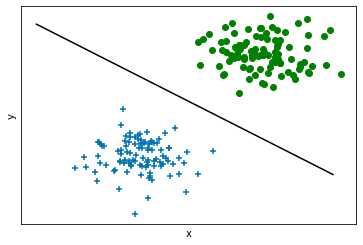
\includegraphics[width=\textwidth]{immagini/4_1/class_linearly_separable.png} 
            \caption{Esempio di dataset linearmente separabile}
            \label{fig:linearly_sep_classification}      
        \end{subfigure}
        \begin{subfigure}[]{0.49\textwidth}
            \centering
            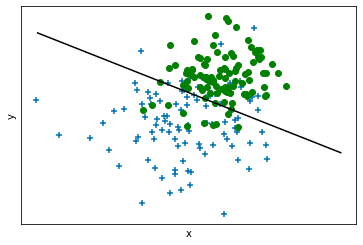
\includegraphics[width=\textwidth]{immagini/4_1/class_non_linearly_separable.png}    
            \caption{Esempio di dataset non linearmente separabile}
            \label{fig:non_linearly_sep_classification}    
        \end{subfigure}
        
    \end{figure}

    Un modello lineare può ad esempio essere utilizzato anche nel contesto dei problemi di classificazione: ad esempio in Figura \ref{fig:linearly_sep_classification} sono rappresentati un insieme di punti appartenenti a due classi (\textit{etichette}) differenti, fornito un dataset di questo tipo l'obiettivo in un problema di classificazione è apprendere una funzione d'ipotesi $h$ che, dato un nuovo punto $(x, y)$, fornisca in output l'etichetta corretta.
    
    In generale si definisce \textit{decision boundary} il piano che separa i punti delle due classi, se tale boundary è, come nell'esempio, una linea retta si parla di classi \textit{linearmente separabili}. Per adattare l'approccio già citato per il caso della regressione al contesto della classificazione semplicemente introduco il concetto di \textit{soglia}: se un determinato elemento assume un valore $> 0$ nella funzione $h$ allora $h(x) = 1$ altrimenti $h(x) = 0$, formalmente posso quindi pensare di far passare il risultato di $h$ in una \textit{funzione di soglia} ed utilizzare tale risultato come classe risultante:
    \[h(\boldsymbol{x}) = \text{Soglia}(\boldsymbol{w} \cdot \boldsymbol{x}) \ \text{con} \ \text{Soglia(z)} = 1 \ \text{se} \ z \geq 0 \ \text{altrimenti} \ 0\]
    Noto come defininendo in questo modo il modello sia non sia però possibile aggiornare i pesi utilizzando lo stesso approccio adottato nel caso della regressione: il gradiente di $h$ è infatti sempre pari a 0 tranne nei punti in cui $\boldsymbol{w} \cdot \boldsymbol{x} = 0$ in cui però è indefinito.
    
    La soluzione è quella di utilizzare la \textit{percepron learning rule}:
    \[w_i \leftarrow w_i + \alpha (y - h(\boldsymbol{x})) x_i\]
    lavorando su problemi di classificazione binaria 0/1 questa regola intuitivamente aggiornerà i pesi solamente nel caso in cui il risultato del modello sia errato, infatti:
    \begin{itemize}
        \item Se l'output è corretto i pesi non vengono aggiornati: $w_i \leftarrow w_i + \alpha \cdot 0 = w_i$
        \item Se $y = 1$ ma $h(\bf{x}) = 0$ allora $w_i$ viene aumentato quando il relativo $x_i$ è positivo e diminuito quando è negativo, in questo modo il prodotto $\boldsymbol{w} \cdot \boldsymbol{x}$ aumenta e la funzione d'ipotesi viene di conseguenza corretta  verso il valore 1.
        \item Se $y = 0$ ma $h(\bf{x}) = 1$ allora $w_i$ viene diminuito quando il relativo $x_i$ è positivo e aumentato quando è negativo, in questo modo il prodotto $\boldsymbol{w} \cdot \boldsymbol{x}$ diminuisce e la funzione d'ipotesi viene di conseguenza corretta verso il valore 0.
    \end{itemize}
    Solitamente questa regola di apprendimento viene applicata un esempio alla volta, estraendo casualmente elementi dal dataset.

    \begin{figure}[H]
        \begin{subfigure}{0.5\textwidth}
            \centering
            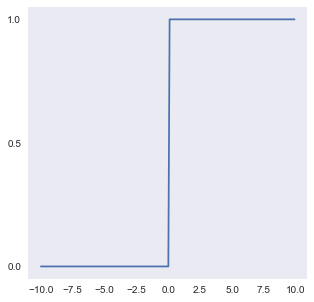
\includegraphics[width=\textwidth]{immagini/4_1/threshold.png} 
            \caption{Funzione Soglia}
            \label{fig:threshold}
        \end{subfigure}
        \begin{subfigure}{0.5\textwidth}
            \centering
            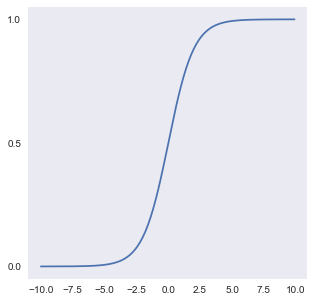
\includegraphics[width=\textwidth]{immagini/4_1/logistic.png}
            \caption{Funzione Logistica}
            \label{fig:logistic}
        \end{subfigure}
        \caption{Grafici della funzioni soglia e logistica.}
    \end{figure}

    Come appena dimostrato quindi utilizzare l'output di un modello lineare come input di una \textit{funzione soglia} permette di adattare l'approccio già utilizzato per il problema della regressione al contesto della classficazione, il principale lato negativo di utilizzare una funzione di questo tipo deriva dal fatto che non è differenziabile, un classificatore basato su una funzione di questo tipo inoltre fornisce sempre valori binari, anche quando il risultato è molto vicino al valore della soglia e nella maggior parte delle situazioni una funzione di questo tipo non è ciò di cui abbiamo bisogno.

    Per i motivi appena descritti spesso si preferisce utilizzare una \textit{funzione logistica} che intuitivamente corrisponde ad una versione \textit{rilassata} della funzione soglia, formalmente è definita come:
    \[ \text{Logistica}(z) = \frac{1}{1 + e^{-z}}\]
    Utilizzando come input il risultato del modello:
    \[h(\boldsymbol{x}) = \text{Logistica}(\boldsymbol{w} \cdot \boldsymbol{x}) = \frac{1}{1 + e^{- \boldsymbol{w \cdot x}}}\]
    Importante notare come l'output della funzione non sia più, come nella funzione soglia, un numero tra 0 e 1, bensì un valore continuo compreso nell'intervallo $[0, 1]$ che può essere interpretato come la probabilità che il punto $\bf{x}$ appartenga all'etichetta 1.

    La funzione logistica ha proprietà matematiche più vantaggiose rispetto alla funzione precedente, prima fra tutte la derivabilità su tutto il dominio, proprietà sfruttata per il processo di aggiornamento dei pesi, che prende il nome di \textit{regressione logistica}. Non esiste, come nella regressione lineare, una soluzione in forma chiusa per trovare in modo analitico l'ottimo del vettore $\bf{w}$, ma posso ancora una volta sfruttare la discesa del gradiente: l'aggiornamento dei pesi avverrà quindi secondo la seguente formula:
    \[w_i \leftarrow w_i - \alpha \frac{\partial}{\partial w_i} L(\boldsymbol{w})\]
    Calcolando la derivata parziale della funzione di perdita (Anche in questo caso quadratica):
    \[\frac{\partial}{\partial w_i} L(\boldsymbol{w}) = -2 (y - h(\boldsymbol{x})) \times h(\boldsymbol{x})(1 - h(\boldsymbol{x})) \times x_i\]
    Posso quindi riscrivere la formula per l'aggiornamento dei pesi:
    \begin{equation}
        w_i \leftarrow w_i + \alpha (y - h(\boldsymbol{x})) \times h(\boldsymbol{x})(1 - h(\boldsymbol{x})) \times x_i
    \end{equation}
    I metodi come la regressione lineare/logistica rimangono comunque fortemente limitati nel tipo di pattern dei dati che possono descrivere, per questo molto spesso si rendono necessari modelli più \textit{espressivi} per  poter approssimare un determinato dataset, modelli di questo tipo prendono il nome di \textit{reti neurali}: modelli complessi basati su circuiti algebrici.

\end{document}